\section{Resultados y An\'alisis}

Tras el montaje del sistema de p\'endulos acoplados y el registro
de las mediciones mediante el sensor Cassy, se recopil\'o un
conjunto de 15 series de datos. Estas series corresponden a tres
condiciones iniciales distintas para cada una de las cinco
configuraciones experimentales estudiadas. Los datos temporales de
los \'angulos de cada p\'endulo fueron procesados utilizando un
c\'odigo en Python, con el fin de generar gr\'aficas de la evoluci\'on
angular $\theta_i(t)$ y, fundamentalmente, para determinar las
frecuencias angulares principales de oscilaci\'on mediante la
aplicaci\'on de la Transformada R\'apida de Fourier (FFT).

En la \cref{tab:frequencies} se presenta un resumen de las
frecuencias angulares principales identificadas para cada p\'endulo,
en funci\'on de la configuraci\'on del sistema y de la condici\'on
inicial aplicada. Un an\'alisis preliminar de estos valores revela
patrones interesantes: la frecuencia angular usual del p\'endulo 2
(el m\'as largo) se sit\'ua consistentemente alrededor de
\qty{0.844}{\Hz}, con una desviaci\'on est\'andar
reducida de \num{0.009}, lo que indica una notable regularidad en su
comportamiento oscilatorio a esta frecuencia.

\begin{table*}[htbp!]
	\centering
	\caption{Frecuencias angulares principales de oscilaci\'on
		($f_i$) identificadas para cada p\'endulo, seg\'un la
		configuraci\'on experimental y las condiciones iniciales aplicadas.
	}
	\label{tab:frequencies}
	\pgfplotstabletypeset[
	every head row/.style={
		before row=\toprule,
		after row=\midrule
	},
	every last row/.style={after row=\bottomrule},
	columns/config/.style={
		string type,
		column name={Configuración},
	},
	columns/mode/.style={
		string type,
		column name={Condición Inicial},
	},
	columns/freq1/.style={
		column name=$f_1 [\si{\Hz}]$,
		fixed,
		fixed zerofill,
		precision=3,
	},
	columns/freq2/.style={
		column name=$f_2 [\si{\Hz}]$,
		fixed,
		fixed zerofill,
		precision=3,
	},
	columns/freq3/.style={
		column name=$f_3 [\si{\Hz}]$,
		fixed,
		fixed zerofill,
		precision=3,
	},
	every nth row={3}{before row=\midrule},
	columns={config, mode, freq1, freq2, freq3}
	]{\datafreq}
\end{table*}

En contraste, para el p\'endulo 1, se identifican dos agrupaciones
principales de frecuencias: una en torno a \qty{1.311}{\Hz}
(desviaci\'on est\'andar de \num{0.019}) y otra cercana a
\qty{0.843}{\Hz} (desviaci\'on est\'andar de \num{0.008}). Un
comportamiento similar, aunque con valores ligeramente distintos, se
observa en el p\'endulo 3, el cual exhibe frecuencias predominantes
alrededor de \qty{1.255}{\Hz} (desviaci\'on est\'andar de \num{0.063})
y \qty{0.843}{\Hz} (desviaci\'on est\'andar de \num{0.008}).
Adicionalmente, para el p\'endulo 3, se detect\'o una frecuencia
excepcionalmente baja de \qty{0.0021}{\Hz}, la cual se present\'o
de manera aislada \'unicamente en la Configuraci\'on 5-1 bajo las
condiciones iniciales (100). La aparici\'on de m\'ultiples
frecuencias dominantes para los p\'endulos laterales (1 y 3)
sugiere la excitaci\'on selectiva de diferentes modos normales del
sistema, cuya manifestaci\'on depende de la configuraci\'on
espec\'ifica de acoplamiento y de las condiciones iniciales
impuestas.

Un an\'alisis m\'as detallado del \cref{tab:frequencies} evidencia
que para la condici\'on inicial (010) (excitaci\'on \'unica del
p\'endulo central), los tres p\'endulos tienden a oscilar con una
frecuencia dominante com\'un o muy similar, independientemente de la
configuraci\'on de acoplamiento. Esto podr\'ia indicar la
excitaci\'on preferente de un modo normal en el que los tres
p\'endulos participan de manera sincronizada. En las dem\'as
condiciones iniciales, el p\'endulo 3 generalmente muestra una
frecuencia principal inferior a la del p\'endulo 1. No obstante,
se observa una excepci\'on en la configuraci\'on 6-6, donde la
frecuencia principal del p\'endulo 3 supera a la del p\'endulo 1.

La menor frecuencia caracter\'istica del p\'endulo 2 se atribuye
principalmente a su mayor longitud y masa (y por ende, mayor momento
de inercia) en comparaci\'on con los p\'endulos laterales. Las
diferencias observadas en las frecuencias principales entre los
p\'endulos 1 y 3, as\'i como su variaci\'on entre las distintas
configuraciones, son consecuencia de c\'omo los diferentes puntos de
acople de los resortes modifican la interacci\'on entre ellos. La
altura a la que se fijan los resortes en las barras de los
p\'endulos influye en la magnitud de los torques de acoplamiento y,
por lo tanto, en la 'rigidez efectiva angular' del acoplamiento
entre cada par de p\'endulos. Esto, a su vez, afecta las
caracter\'isticas de los modos normales del sistema. La
configuraci\'on 6-6, por ejemplo, debido a sus puntos de acople
espec\'ificos, facilita un tipo de interacci\'on que
favorece un modo donde el p\'endulo 3 oscila a una frecuencia mayor
que el 1, a diferencia de otras geometr\'ias de acople.
Esta sensibilidad a la posici\'on del acople tambi\'en es relevante
para interpretar la frecuencia excepcionalmente baja de
\qty{0.0021}{\Hz} previamente identificada en el p\'endulo 3 para la
configuraci\'on 5-1 con condici\'on inicial (100). En dicha
configuraci\'on, uno de los puntos de anclaje del resorte est\'a
muy pr\'oximo al pivote, lo que resulta en una 'rigidez efectiva
angular' muy d\'ebil para ciertos patrones de movimiento, lo que
consecuentemente lleva a la aparici\'on de frecuencias de
oscilaci\'on extremadamente bajas para el modo asociado.

Finalmente, es de destacar el caso de la configuraci\'on 6-4 bajo la
condici\'on inicial (100), donde ambos p\'endulos laterales (1 y 3)
presentan la misma frecuencia principal. Esta igualdad podr\'ia ser
indicativa de la excitaci\'on de un modo normal con un alto grado de
simetr\'ia en el movimiento de los p\'endulos externos.

\subsection*{Frecuencias del Modelo Teórico}

Al resolver el problema de valores propios para el sistema representado
en forma matricial, \cref{eq:matrix-form}, se obtuvieron las
frecuencias te\'oricas de los modos normales para cada una de las
cinco configuraciones experimentales. Estos resultados se presentan
en la \cref{tab:theoric-freq}. Como es de esperar para un sistema
con tres grados de libertad, se identifican tres frecuencias de modo
normal distintas para cada configuraci\'on.

Los valores te\'oricos en la \cref{tab:theoric-freq}
sugieren una tendencia general donde una mayor distancia entre el
punto de acople del resorte y el pivote del p\'endulo tiende a
correlacionarse con un aumento en las frecuencias de los modos normales.
En cuanto a los valores espec\'ificos, se observa
con regularidad una frecuencia te\'orica cercana a \qty{0.8}{\Hz},
as\'i como otras agrupadas en torno a \qty{1.3}{\Hz} y, en algunos
casos, pr\'oximas a \qty{1.6}{\Hz}.

Es importante destacar que las frecuencias te\'oricas obtenidas, en
general, no difieren significativamente de los valores experimentales
predominantes que fueron presentados en la \cref{tab:frequencies}.
La notable excepci\'on es la frecuencia experimental an\'omalamente
baja de \qty{0.0021}{\Hz} (identificada previamente en la
Configuraci\'on 5-1, condici\'on inicial (100) para el p\'endulo 3),
la cual no tiene una contraparte directa en el espectro te\'orico
calculado. No obstante, la concordancia general para las dem\'as
frecuencias principales sugiere que el modelo te\'orico linealizado,
basado en la aproximaci\'on de peque\~nas oscilaciones, logra
aproximar razonablemente el comportamiento din\'amico del sistema
experimental construido.

\begin{table*}[htbp!]
	\centering
	\caption{Frecuencias te\'oricas de los modos normales ($f_{0i}$)
		calculadas para el sistema, seg\'un la configuraci\'on de
		acoplamiento.
	}
	\label{tab:theoric-freq}
	\pgfplotstabletypeset[
	every head row/.style={
		before row=\toprule,
		after row=\midrule
	},
	every last row/.style={after row=\bottomrule},
	columns/config/.style={
		string type,
		column name={Configuración},
	},
	columns/f2/.style={
		column name=$f_{01} [\si{\Hz}]$,
		fixed,
		fixed zerofill,
		precision=3,
	},
	columns/f1/.style={
		column name=$f_{02} [\si{\Hz}]$,
		fixed,
		fixed zerofill,
		precision=3,
	},
	columns/f3/.style={
		column name=$f_{03} [\si{\Hz}]$,
		fixed,
		fixed zerofill,
		precision=3,
	},
	columns={config, f2, f1, f3}
	]{\theoric}
\end{table*}

En la \cref{tab:comparison} se presenta una comparaci\'on directa
entre las frecuencias experimentales ($f_\text{ex}$) predominantes,
identificadas para cada modo normal discernible en las distintas
configuraciones, y sus correspondientes frecuencias te\'oricas
($f_\text{te}$). La tabla tambi\'en incluye el error relativo
porcentual, calculado como
$\mid \left(1 - \frac{f_\text{te}}{f_\text{ex}}\right) \mid 100\%$,
para cuantificar la discrepancia.

Los errores relativos porcentuales var\'ian considerablemente.
El error m\'as grande observado, sin considerar la frecuencia
an\'omala de \qty{0.0021}{\Hz} que no se incluye en esta
comparaci\'on directa de modos, es del \qty{2.509}{\percent}. Por
otro lado, el error m\'as bajo registrado es de tan solo
\qty{0.036}{\percent}. Estos valores indican que, si bien existen
desviaciones, el modelo te\'orico es capaz de predecir las
frecuencias de los modos normales con un grado de precisi\'on
generalmente alto para la mayor\'ia de los casos estudiados.

\begin{table*}[htbp!]
	\centering
	\caption{Comparaci\'on entre las frecuencias experimentales
		predominantes ($f_\text{ex}$) y las frecuencias te\'oricas
		($f_\text{te}$) para los modos normales, junto con el error
		relativo porcentual.
	}
	\label{tab:comparison}
	\pgfplotstabletypeset[
	every head row/.style={
		before row=\toprule,
		after row=\midrule
	},
	every last row/.style={after row=\bottomrule},
	columns/config/.style={
		string type,
		column name={Configuraci\'on},
	},
	columns/fe/.style={
		column name=$f_\text{ex} [\si{\Hz}]$,
		fixed,
		fixed zerofill,
		precision=3,
	},
	columns/ft/.style={
		column name=$f_\text{te} [\si{\Hz}]$,
		fixed,
		fixed zerofill,
		precision=3,
	},
	columns/err/.style={
		column name={Error Relativo $[\%]$},
		fixed,
		fixed zerofill,
		precision=3,
	},
	every nth row={3}{before row=\midrule},
	columns={config, fe, ft, err}
	]{\comparison}
\end{table*}

\subsection*{Casos Representativos de Oscilaci\'on y Espectros de Frecuencia}

A partir del conjunto de datos experimentales recopilados, se
seleccionaron seis casos considerados como los m\'as representativos
de los diversos comportamientos din\'amicos observados en el sistema
de p\'endulos acoplados. Para cada uno de estos casos seleccionados,
se presentan figuras que ilustran de manera conjunta: (a) la
evoluci\'on tempo ral del desplazamiento angular $\theta_i(t)$ de los
p\'endulos involucrados y (b) el correspondiente espectro de
amplitudes obtenido a partir de la FFT de dichas series temporales.
Estas representaciones gr\'aficas se encuentran detalladas en las
\cref{fig:111-11,fig:010-51,fig:101-61,fig:010-62,fig:100-66,fig:010-66}.

\begin{figure}[htbp!]
	\centering
	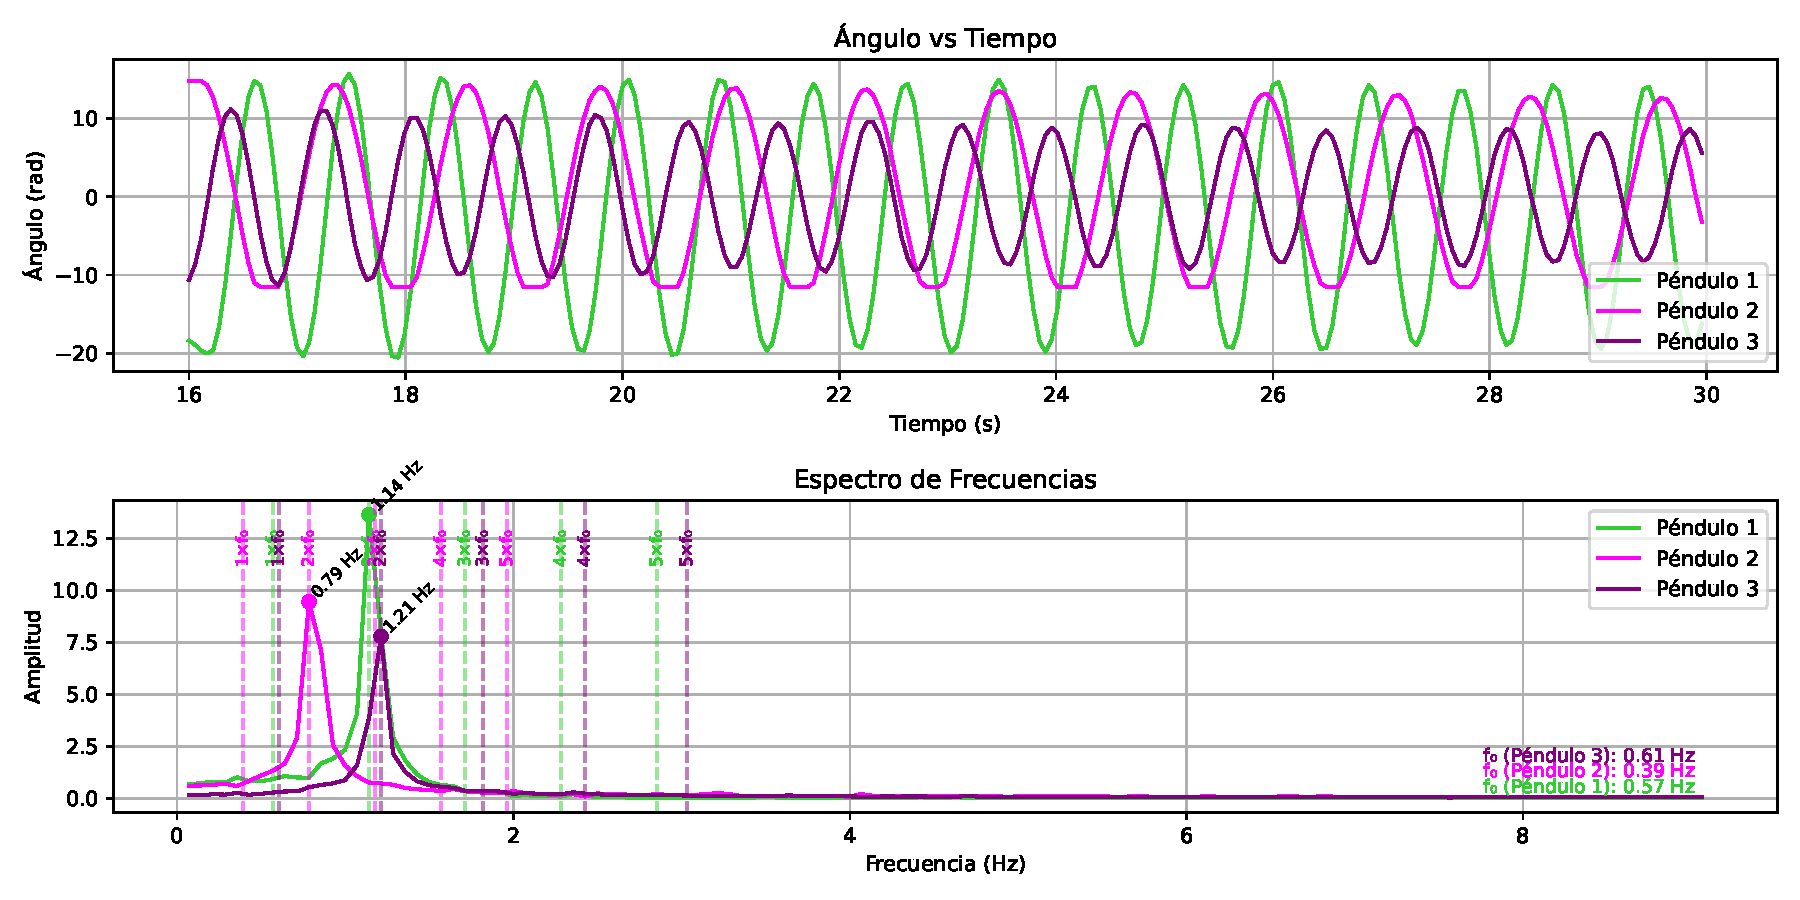
\includegraphics[width=\linewidth]{./Figures/111_11_filtrado.pdf}
	\caption{Evoluci\'on temporal del desplazamiento angular y espectro de
		frecuencias (FFT) para la Configuraci\'on 1-1 con condiciones
	iniciales (111).}
	\label{fig:111-11}
\end{figure}

\begin{figure}[htbp!]
	\centering
	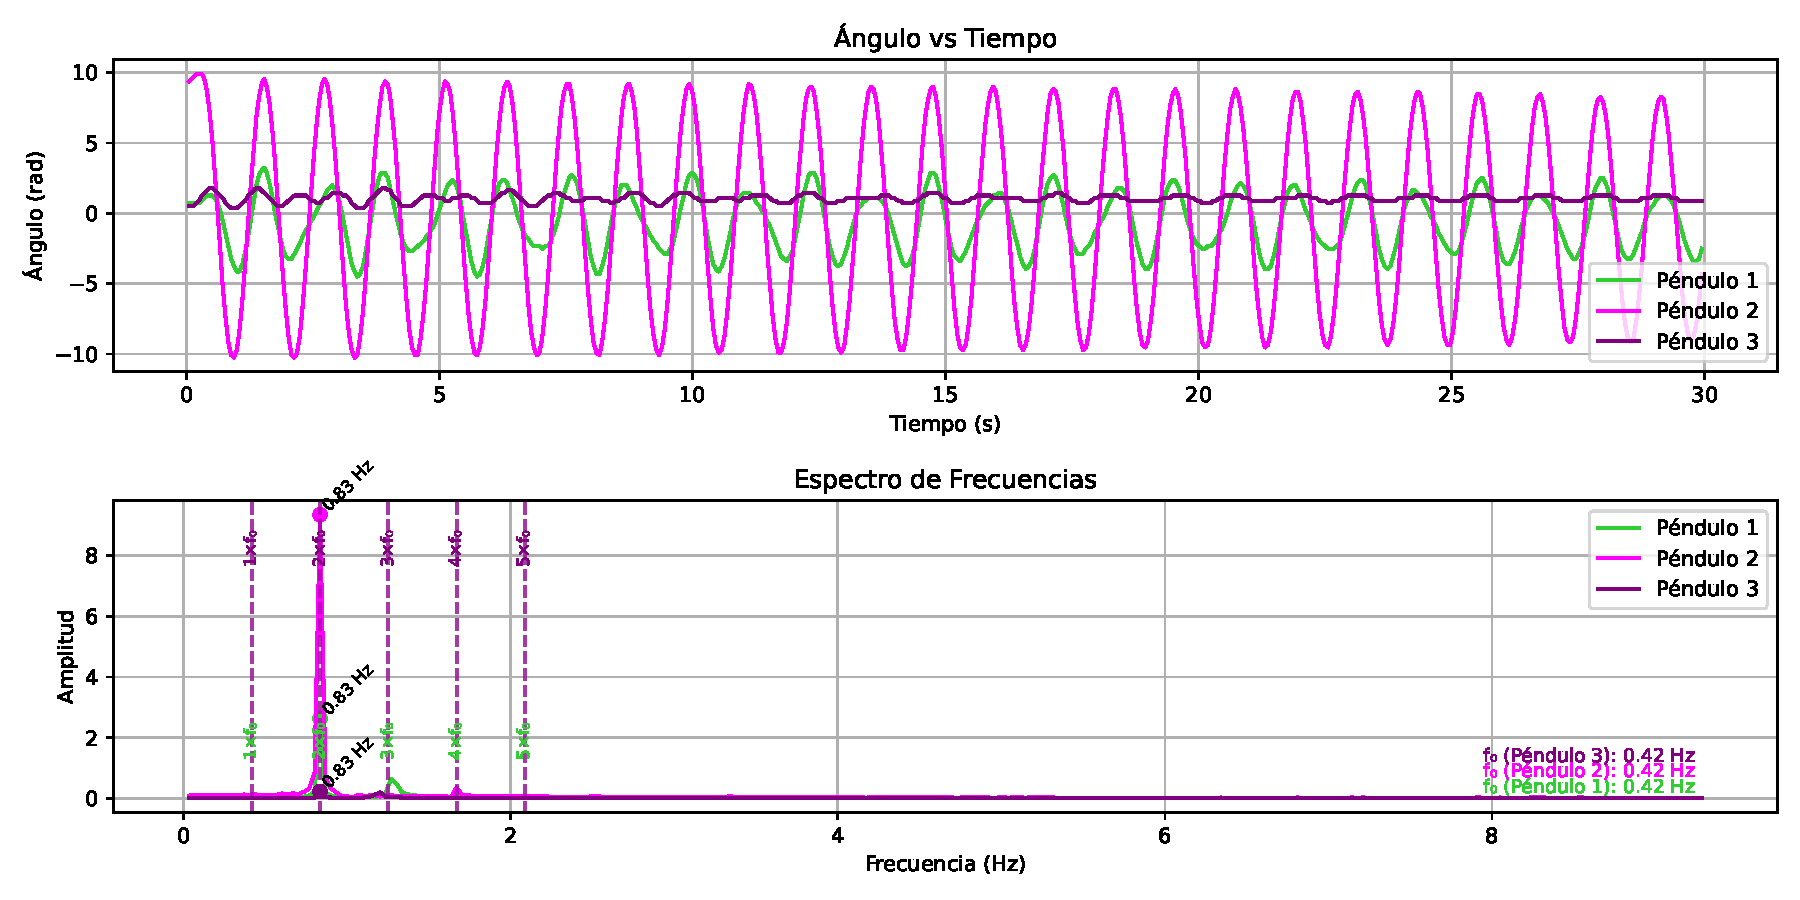
\includegraphics[width=\linewidth]{./Figures/010_15_filtrado.pdf}
	\caption{Evoluci\'on temporal del desplazamiento angular y espectro de
		frecuencias (FFT) para la Configuraci\'on 5-1 con condiciones
	iniciales (010).}
	\label{fig:010-51}
\end{figure}

\begin{figure}[htbp!]
	\centering
	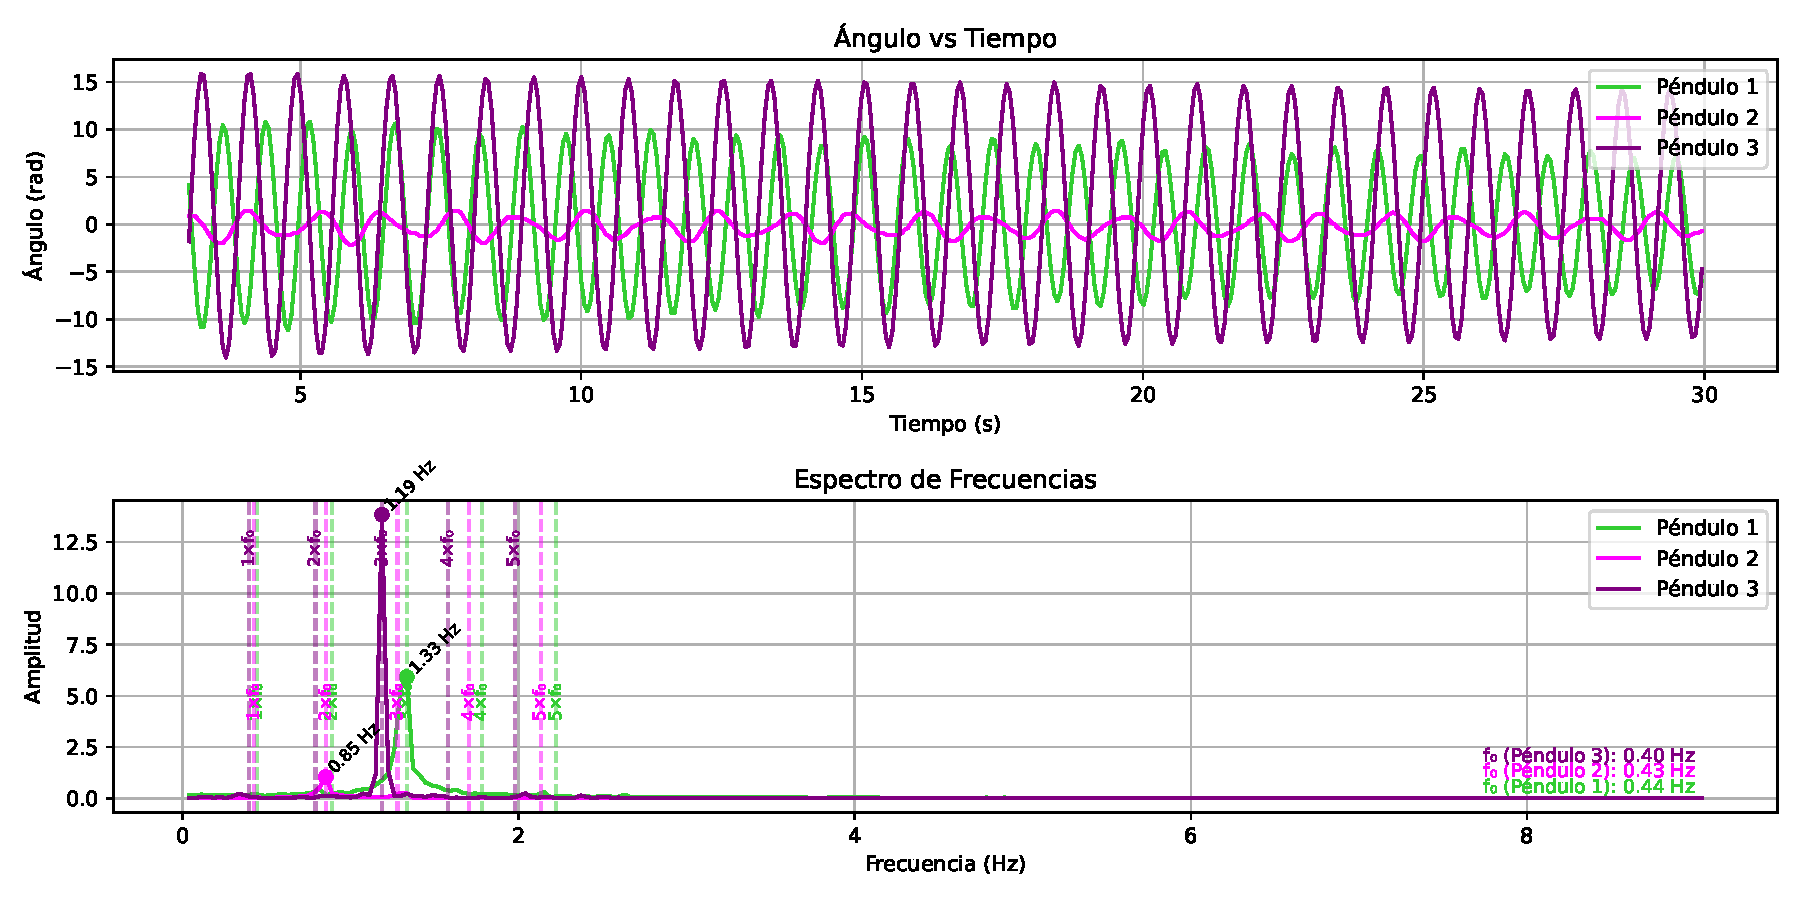
\includegraphics[width=\linewidth]{./Figures/101_16_filtrado.pdf}
	\caption{Evoluci\'on temporal del desplazamiento angular y espectro de
		frecuencias (FFT) para la Configuraci\'on 6-1 con condiciones
	iniciales (101).}
	\label{fig:101-61}
\end{figure}

\begin{figure}[htbp!]
	\centering
	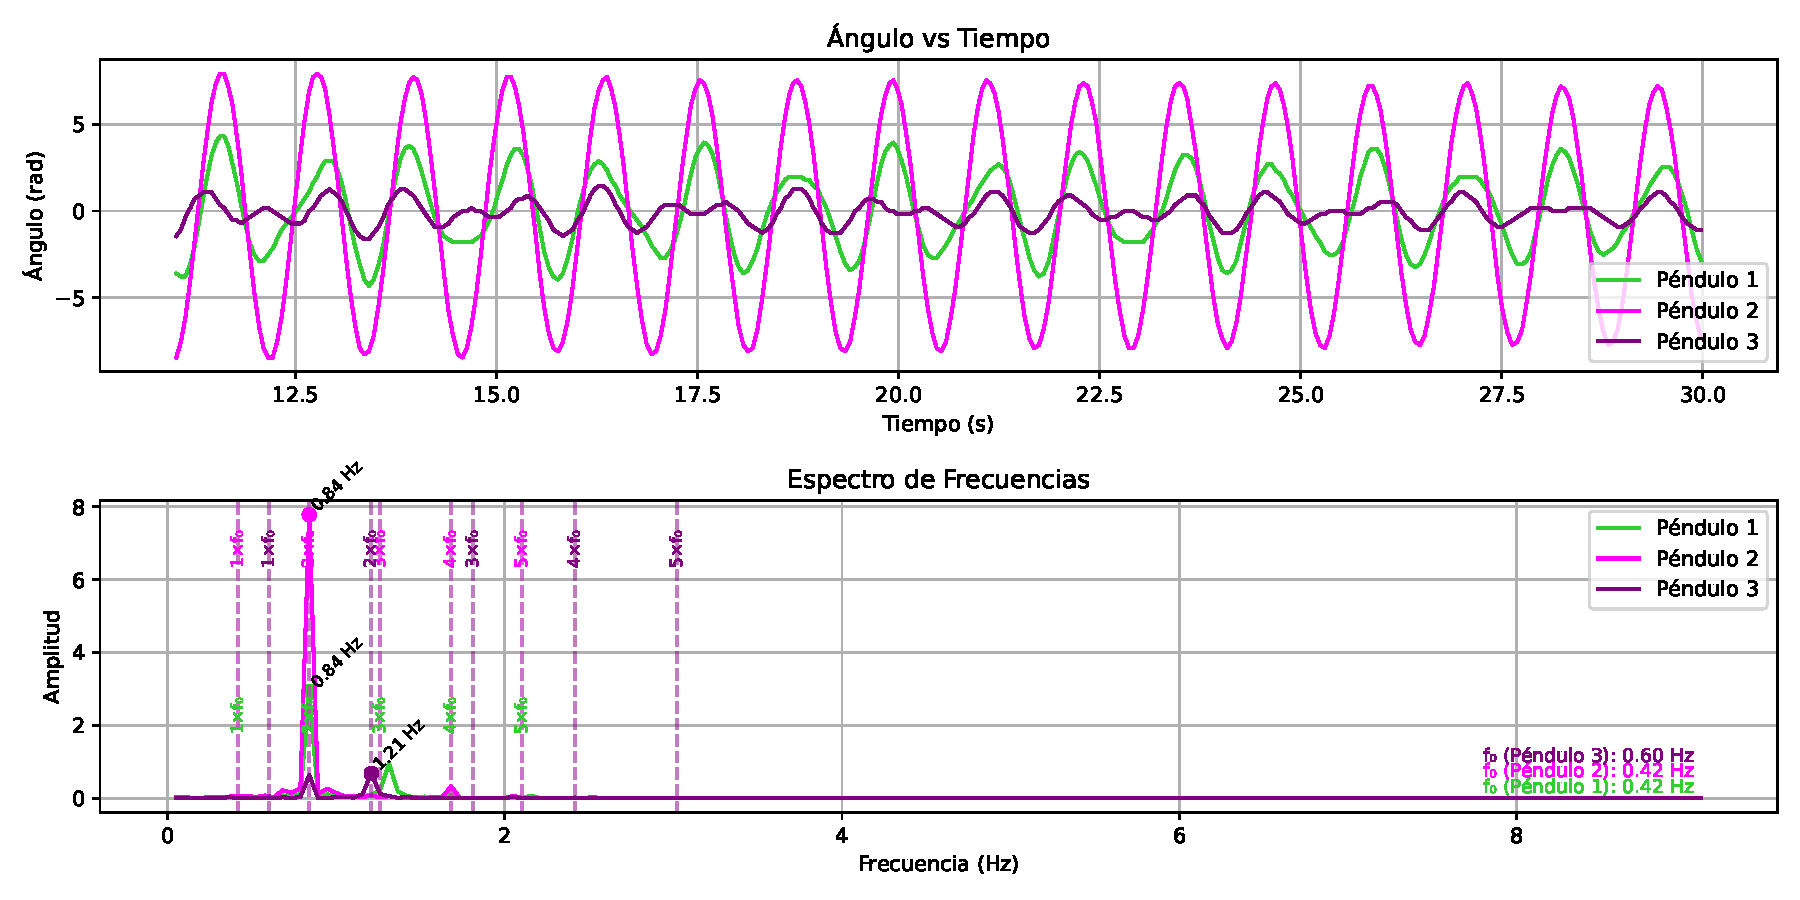
\includegraphics[width=\linewidth]{./Figures/010_26_filtrado.pdf}
	\caption{Evoluci\'on temporal del desplazamiento angular y espectro de
		frecuencias (FFT) para la Configuraci\'on 6-2 con condiciones
	iniciales (010).}
	\label{fig:010-62}
\end{figure}

\begin{figure}[htbp!]
	\centering
	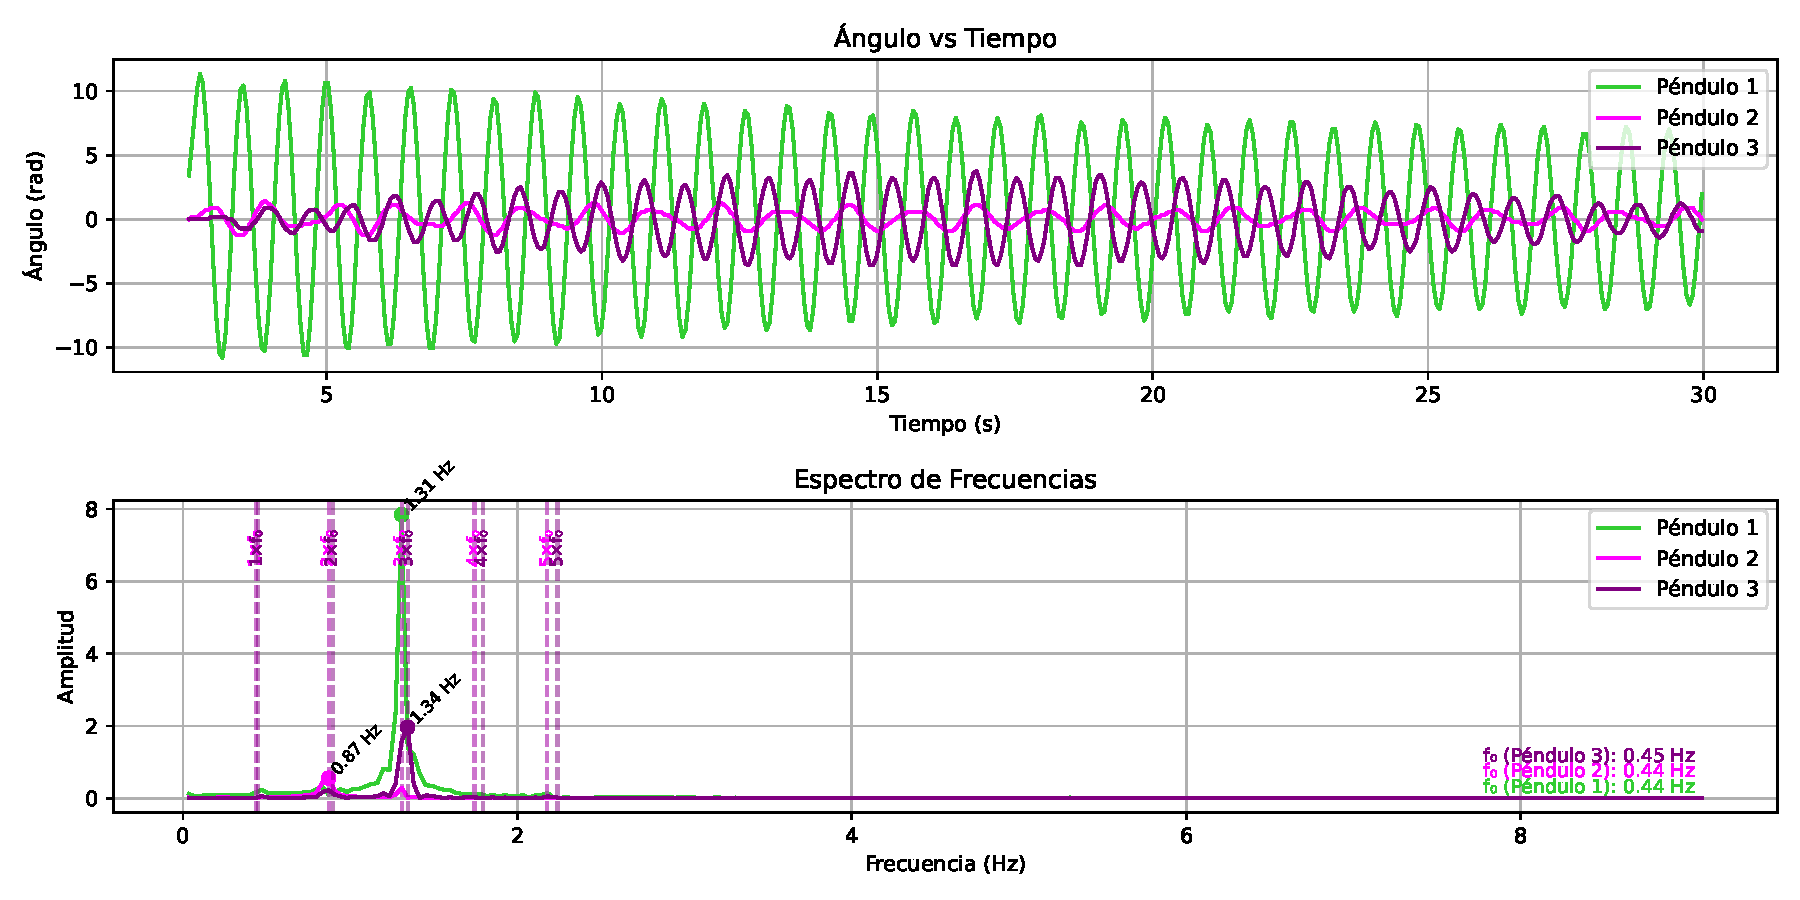
\includegraphics[width=\linewidth]{./Figures/001_66_filtrado.pdf}
	\caption{Evoluci\'on temporal del desplazamiento angular y espectro de
		frecuencias (FFT) para la Configuraci\'on 6-6 con condiciones
	iniciales (100).}
	\label{fig:100-66}
\end{figure}

\begin{figure}[htbp!]
	\centering
	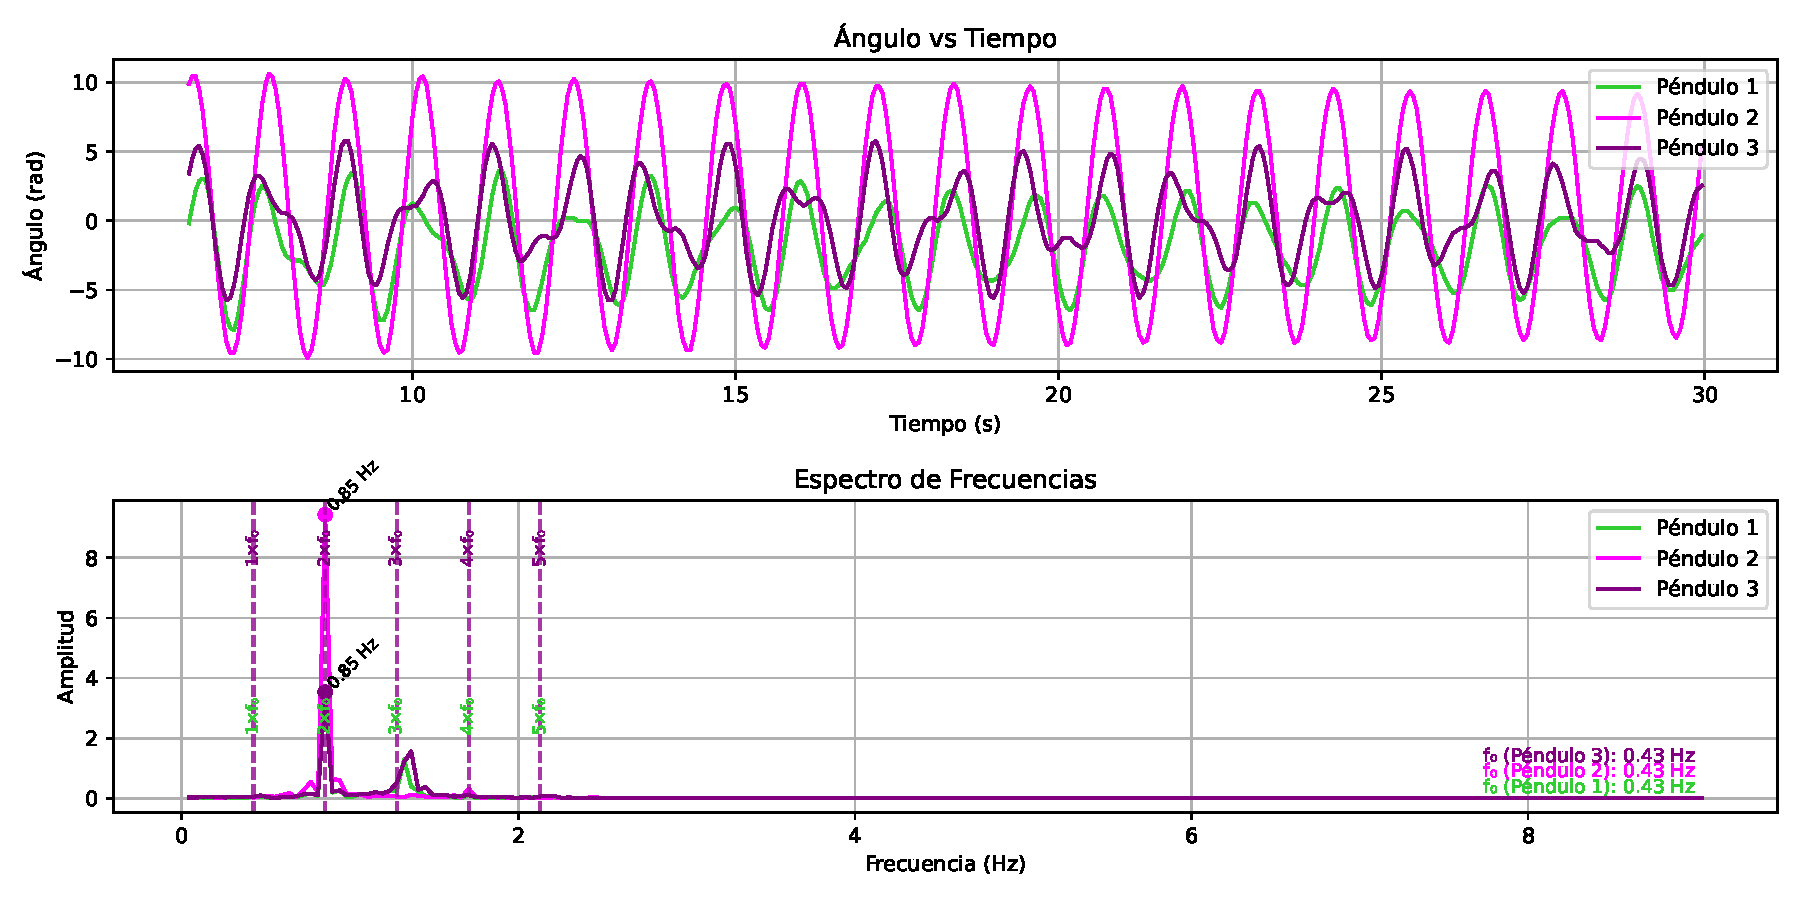
\includegraphics[width=\linewidth]{./Figures/010_66_filtrado.pdf}
	\caption{Evoluci\'on temporal del desplazamiento angular y espectro de
		frecuencias (FFT) para la Configuraci\'on 6-6 con condiciones
	iniciales (010).}
	\label{fig:010-66}
\end{figure}

En la \cref{fig:111-11}, correspondiente a la Configuraci\'on 1-1 con
condiciones iniciales (111), se observa que cada p\'endulo exhibe un
pico de frecuencia principal distintivo en su espectro FFT, sin
compartir una \'unica frecuencia dominante com\'un. Estos picos
espectrales son relativamente anchos, lo que sugiere una duraci\'on
efectiva de coherencia limitada para estas oscilaciones o la
presencia de un amortiguamiento significativo. Dicho amortiguamiento
es esperable debido a las interacciones inherentes entre los
p\'endulos (acoplamiento y fricci\'on) y se ve acentuado por la
complejidad del movimiento resultante de las condiciones iniciales,
donde los p\'endulos laterales se excitan desfasados respecto al
central. Particularmente, el comportamiento temporal del p\'endulo 2
en este caso se desv\'ia de un movimiento arm\'onico
simple, presentando modulaciones en su amplitud.

En contraste, la \cref{fig:010-51} (Configuraci\'on 1-5, condiciones
iniciales (010)) muestra picos espectrales considerablemente m\'as
definidos y estrechos, indicativo de un comportamiento m\'as regular
y menos amortiguado para las frecuencias dominantes. Notablemente,
los tres p\'endulos comparten la misma frecuencia principal,
reafirmando la tendencia observada para la condici\'on (010). Adem\'as
de la frecuencia fundamental, se aprecian componentes espectrales
secundarias comunes a los tres p\'endulos, aunque con diferentes
amplitudes relativas; por ejemplo, el p\'endulo 2 podr\'ia dominar en
amplitud en un arm\'onico secundario, mientras que el p\'endulo 1 lo
har\'ia en otro. En este caso, el p\'endulo 3 parece exhibir una
menor amplitud en sus componentes espectrales, lo que podr\'ia
atribuirse a una transmisi\'on de energ\'ia menos eficiente hacia \'el
debido a la geometr\'ia espec\'ifica de los puntos de acople en esta
configuraci\'on. La evoluci\'on temporal de los \'angulos para este
caso (\cref{fig:010-51}) es m\'as estable y coherente, con una
disminuci\'on gradual de las amplitudes generales debido al
amortiguamiento residual.

Para la Configuraci\'on 6-1 bajo condiciones iniciales (101),
ilustrada en la \cref{fig:101-61}, el an\'alisis espectral revela
nuevamente tres picos de frecuencia principales distintos, sugiriendo
la excitaci\'on de m\'ultiples modos normales. El p\'endulo 3 muestra
una mayor amplitud en su frecuencia principal y un pico espectral
m\'as estrecho en comparaci\'on con el p\'endulo 1. Esta
caracter\'istica podr\'ia estar relacionada con la naturaleza del
acoplamiento en esta configuraci\'on particular y el hecho de que el
p\'endulo 3 es uno de los excitados inicialmente (condici\'on (101)).

Por otro lado, el p\'endulo 2 presenta oscilaciones de amplitud muy
reducida, un comportamiento consistente con la excitaci\'on de un
modo normal donde los p\'endulos laterales se mueven de forma
predominantemente desfasada y el p\'endulo central tiene una
participaci\'on m\'inima. Adicionalmente, en la evoluci\'on temporal
se observa un intercambio de energ\'ia entre los p\'endulos 1 y 3:
leves aumentos en la amplitud de oscilaci\'on del p\'endulo 3 tienden
a coincidir con disminuciones en la amplitud del p\'endulo 1, y
viceversa. Este fen\'omeno es caracter\'istico de las pulsaciones
(batidos) en sistemas acoplados y es esperable si las frecuencias
de los modos que involucran principalmente a estos dos p\'endulos son
cercanas y hay una transferencia de energ\'ia entre ellos, en un
contexto de conservaci\'on aproximada de la energ\'ia (descontando
p\'erdidas por fricci\'on).

Para la configuraci\'on 6-2 bajo la condici\'on inicial (010),
ilustrada en la \cref{fig:010-62} (no incluida en el presente
documento, pero referenciada para an\'alisis), el espectro del
p\'endulo 2 muestra una frecuencia principal con una amplitud
prominente y un pico espectral estrecho en comparaci\'on con otras
componentes secundarias. Entre estas \'ultimas, se identifica un pico
cuya frecuencia es aproximadamente cuatro veces la frecuencia
principal, aunque su contribuci\'on en amplitud es mucho menor.
Debido a esta marcada dominancia de la frecuencia fundamental, el
comportamiento temporal del p\'endulo 2 se asemeja de forma notable
a un movimiento arm\'onico simple. En cuanto al p\'endulo 1, este
comparte la frecuencia principal observada en el p\'endulo 2; sin
embargo, su espectro tambi\'en exhibe otro pico significativo a una
frecuencia ligeramente superior al triple de la fundamental. Esta
composici\'on multifrecuencial indica que el movimiento del p\'endulo
1 no es estrictamente arm\'onico simple, aunque s\'i manifiesta una
clara periodicidad, como se evidencia en su evoluci\'on temporal.
Finalmente, el p\'endulo 3 presenta en su espectro dos picos con
amplitudes comparables, cuyas frecuencias se corresponden
aproximadamente con los valores te\'oricos esperados de \qty{0.83}{\Hz}
y \qty{1.2}{\Hz} para los modos involucrados. No obstante, las
amplitudes de estos picos para el p\'endulo 3 son relativamente
bajas, lo que se traduce en una oscilaci\'on de escasa magnitud para
este p\'endulo en particular.

Por \'ultimo, se analiza la configuraci\'on 6-6 con la condici\'on
inicial (100) (excitaci\'on inicial \'unicamente del p\'endulo 1).
En este caso, se observa c\'omo la geometr\'ia de acople facilita una
efectiva transmisi\'on de energ\'ia entre los p\'endulos. El an\'alisis
espectral revela que los tres p\'endulos comparten componentes de
frecuencia en las mismas ubicaciones espectrales. Espec\'ificamente,
los p\'endulos 1 y 3 comparten una frecuencia principal com\'un (m\'as
alta), mientras que el p\'endulo 2 tiene su propia frecuencia
principal a un valor menor. A pesar de ello, el p\'endulo 2 tambi\'en
exhibe picos secundarios en las frecuencias donde los p\'endulos
laterales oscilan predominantemente, indicando su participaci\'on en
esos modos de mayor frecuencia. Este comportamiento, donde todos los
p\'endulos oscilan de manera significativa, distingue a esta
combinaci\'on de configuraci\'on y condici\'on inicial de otras
pruebas hipot\'eticas con la misma condici\'on (100) pero diferentes
puntos de acople, resaltando as\'i el papel determinante de la
posici\'on de los acoples en la din\'amica del sistema.
